%Present implementation details, program structure etc.  Further, interesting
%algorithms and data structures should be presented here.
\chapter{Implementation and detailed design} %Carsten
Like Java's main function, Arduino has two special functions: {\tt setup} and {\tt loop}. The former is called once on program start, while the latter is repeatably called
until the Arduino is turned off.\footnote{At least, we haven't discovered a way
to terminate a sketch.}\\ This isn't a very optimized structure. It forces us
to use global variables if we want to reuse anything from setup in loop. Our
solution was to leave {\tt loop} empty and put an endless loop in {\tt setup}
instead. All of our variables could become local with this change, greatly
reducing code size.\\

\section{Setup}
Precalculations

\section{Loop} %Carsten
The loops first manages all props and then checks whether the game is over. First it updates all units AI, where they decide what to do in this frame. The hero is part of this loop and updated as if he had AI, but instead converts player input into actions. After this, all attacks generated from this AI update is executed. This involves all props, where units are checked if they die and coins are if they are collected. Finally the physics is updated, and all props move according to their internal velocities. Minotaurs may update their AI in case a collision function is called.\\ dTime...

\section{Logic} %Carsten
The units needs to receive map data and send actions. This is the {\tt Logic} class' function. It contains numerous methods to calculate a units' surroundings and also handles collision, physics engine, coin collection and attacks.\\
Props can only collide with the map geometry, not with each other. It was not a priority to collide props with each other. Enemies should be able to pass each other and the hero would be damaged when colliding with them in any case. Collision is calculated in straight lines, and only at one axis at a time. This makes long diagonal movement inaccurate, since it is calculated as if the prop moved first horizontally and then vertically. A better collision detection was a possibility, but eventually not prioritized. Collisions are calculated according to rectangular hitboxes.\\
After these simplifications, the collision algorithm is very simple. Given a prop and a distance, it checks each tile in order which the prop will pass through according to its hitbox. If any of the tiles are solid, the prop only travels up to the solid tile and the algorithm terminates. When updating the physics engine, either the {\tt collisionX} or {\tt collisionY} functions are called, used in AI for units or bounce in coins.\\
A linked list of attacks between frames is kept. Units add their attacks to the list during AI updates and the list is cleared after the attacks have been executed. Executions goes through each prop and checks whether the attack hits or not, calling the {\tt hit} function in case it has. Attacks are a separate object, containing damage, push force, the owner and the area. The attacks are only instantiated once at unit instantiation, which only manipulates the area when reusing the attack, thus optimizing on computing time, though costing memory.\\
There is a circular reference, since units require logic which requires scene which in turn requires units. This resulted in forward declarations in scene which is a bit inelegant. It was difficult to design a structure which did not have any circles, since the actors act upon the scene, and the scene returns data to the actor.

\section{Actors}
Units are a subclass of prop, reusing all physics related functions and fields.

\subsection{Enemies}
AI; hunting\\
Currently the only type of enemy is the minotaur, though the current framework was built to contain multiple types.

\subsection{Hero}
Movement

\section{Scenes} %Carsten
Scenes are the objects Containing the map data and all props within. The map is a simple two-dimensional array. The element at two given indexes corresponds to a tile, which has coordinates equal to the two given indexes times the size of a tile. This means world- can easily be converted to tile coordinates or vice versa.\\ In addition to the map, the scene also contain all props, which is the hero, minotaurs and coins. It stores this in two places: in dynamic linked lists, and in arrays. The former is for
dynamic removal of the props, when the coins are collected or the minotaurs are killed. These are used when updating gameplay, to make sure that unused props are not updated, increasing framerate. The latter is for storing all available props , used at map generation. The arrays have a couple of advantages. First they create all used props of each type initially, reusing the same minotaurs and coins in each map. This shortens time needed to allocate and deallocate memory. Additionally, if the amount of props is initially within Arduino's memory bounds, then the maps will never cause the Arduino to run out of memory, since it never allocates more. The obvious drawbacks is that we are limited in the amount of props we need, and that removing any props during play does not increase available memory. The second drawback isn't that much of a problem though, since very little is needed during play.\\ Currently, because of an implementation bug, the props are dynamically allocated, even though they shouldn't need be.
%Additional possible datastructures?
\subsection{Generator} %Carsten
Map generation is executed at setup and whenever the game ends (either by player death or win). The method {\tt newScene} generates a new map with matching points at the entrance and exits. Arduino's programming language does not support returning more than one value, so the method manipulates given pointers instead like in C programming. The new map data overwrites the old one to save time and space, so the given {\tt scene} argument is a pointer to the old scene.  Reusing it saves us from instantiating a new one and deallocating the old one.  We ar not interested in reusing the actual map data, since the player cannot revisit prior levels.\\
The actual algorithm is in three parts: clearing, modulation and generation. First it clears the old map data, setting all tiles to {\tt NONE}, to make sure nothing is left over from the old map. This may be a bit expensive on the processing time considering it is superfluous if the generator works correctly. The reason is a design choice which will be apparent when we reach the generation.\\ %Picture of Modules?
Modulation in this case means separating the map into \emph{modules}\footnote{As opposed to vary the pitch in a voice}. This is where the layout of the map is decided. A module is a small map in itself, in our case a 5x5 map of tiles.  These have been designed by hand and hard-coded into the generator. Every map is construed of a grid of modules, in our case 4x4. The modules are differentiated by which sides one can access it from.  By this we mean the player can traverse from and to this module from the given sides.  The types are left-right (corridor), left-right-up (T-up), left-right-down (T-down), all (cross) and none (closed). A module in the category left-right is guaranteed to have an exit left and right, and may have an exit up or down.\\
The algorithm first instantiates a grid of empty modules, and randomly assigns one of the bottom modules to be a corridor and the entrance. This is the beginning of the solution path, which guarantees that the map can be completed by the player. From then on it picks a direction, left or right, randomly. From then on the algorithm randomly either moves according to its direction or up. When moving sideways the newly visited grid space is assigned to be a corridor. If it hits the edge of the map it moves upwards and changes direction instead. Whenever the solution path moves upwards, the algorithm has to change the space it is in first. If it is in a corridor tile, it changes it to a T-up, and if it is a T-down it changes it to a cross module. Both of these are the same as their predecessors, but with a guaranteed top-side exit. The newly visited module is assigned a T-down module. The algorithm picks a new direction at random (only if it is not at an edge.) and can start the over again. When it attempts to move upwards while at the top, it instead places the exit in the current tile and terminates. All unvisited grid spaces are assigned closed modules, and are not part of the solution path. Thus we have reached a map which has a guaranteed solution.\\
Lastly the program generates the map. This step reads each module in the newly generated grid, randomly picks a module of the specified type, and fills it into the actual map. If it is currently in an entrance or exit room, it places the corresponding door. It changes the original given entrance and exit pointers to
point at the now created door.\\
Every module overlap with a single row or column with all surrounding modules. Overlapping follows a priority of tiles, where the algorithm determines which tile from the modules is used. Platforms are placed before empty tiles, and solid tiles are placed before platforms. This has several benefits. Firstly the maps are more unique since pairs of modules also differ, and makes the seams of modules harder to notice. Secondly, it ensures that upward exits are easier guaranteed since platforms can be placed closer to the upper floors. This is the reason we need to clear the map prior to generation: the old tiles would disrupt this priority, since the algorithm would not be able to discern what is old and what is new during
generation.\\
Old version (nondeterministic time)

\section{Optimization}%Cebrail
The biggest challenge has been the code size due to the low capacity of the flash memory.  The flash memory has a capacity of 32Kb. The first 4.242Kb is reserved for the bootloader and we are limited to go no further than 28.672Kb all inclusive. So we are actually only allowed to upload 24.430Kb of our own code. It may sound fair comparing to what have been achieved with old game consoles, but it became very quick a headache.\\
Every time we compiled our code, we felt like the code was growing exponentially and we reached the limit quicker than we expected, the intern libraries and our code generally took way too much space. Please see Figure~\ref{fig:code_size} for a history of our code size.

From the start, we wrote the code with optimization in mind, but also tried to keep the code maintainable. When we reached the limit, we had to optimize it further, not just to create space for existing code, but also for further additions to the game. Our first step to solve this problem, we analyzed our code and found the main reasons for this occasion, which are described below.

%\begin{enumerate} \item Inefficient datatypes.  \item Unused functions \item
%    Global Variable instead of local.  \item Code verbose.  \item Repeated
%    statements.  \item Getters/Setters.  \item Dependencies.  \item Libraries.
%  \end{enumerate}

\subsubsection{Inefficient datatypes}
A good place to start was the datatypes. Converting the bigger datatypes
to some smaller ones was a easy optimization. Mostly, it was integers that
was converted to data types like {\tt char}, {\tt byte} and {\tt word}.
Which {\tt char} is capably of encoding numbers from -128 to 127. While
{\tt bytes} is a 8-bit unsigned number, from 0 to 255 and {\tt word} is
basically an unsigned 16-bit number, from 0 to 65535. Notice that {\tt byte}
is the unsigned version of {\tt char}. More details in arduinos site\footnote{http://arduino.cc/en/Reference/HomePage}.
\subsubsection{Unused functions}
\subsubsection{Global to local}
A global variable ensures that all the
functions in the class has access to the variable. But there are downsides
to this, it uses more space than local variables and it also increases the chances
of changing the variable value by other functions without intentions. So we changed
the global variables into local variables by declaring and initializing them in the
functions they are going to be used. So it is a matter of declaring them in the right
scopes.
\subsubsection{Code verbose}
\subsubsection{Repeated statements }
Repeated statements - well it speaks for itself. Repeating something that has been calculated
before is just a waste of code space. Simplifying the code in this manner is sometimes
not easy, it requires that you think creative. It often requires you to think - is this
needed? It may not always be obvious. Often it is about finding a shortcut to some
calculation and taking advantage of already existing results.

\subsubsection{Accessor methods}
Accessor methods are getters and setters functions, that make
variables available to other functions. These functions has to
be declared public in the header file on order to be visible to the
other files. But we found out that these functions are more inefficient
compared to public variables. So we deleted these functions
and made the variables public.

\subsubsection{Dependencies}

\subsubsection{Libraries}
The libraries are the most space allocating part of code. Both our external and
our internal libraries fill much of the code. The internal libraries are
inclusions of our own written code, everything from logic to units. The external
libraries contains which are necessary to communicate with the EEPROM,
Gameduino 2 and Wii nunchuk.

\subsection{Code Size bloat} Bootloader GD2 includes \subsection{Further
optimization} Custom written or shortened extern libraries

\subsection{Inconsistencies} %Carsten


\section{Game loop} Essentially the game is one long loop, which ends whenever
the game does. Each iteration executes the gamelogic per frame, such as moving
the player and monsters around. Gameloops vary from simple while(true) loops
to dynamic separate gameloops handling separate calculations (such as
separating rendering from gameplay).For this we only needed a simple game
loop, updating the world in each iteration. To ensure a consistent gameplay
experience, we needed to know how much time passes betweenframe updates.
Without this, the game would run faster or slower on different processors or
inconsistently in different ingame events, throwing off the players’ sense of
timing. For example, the game would be equally playable with either 30 or 60
frames per second. If the difference isn’t incorporated in the gamelogic
though,the game would run twice as fast with 60 frames per second! Our
implementation of a frames per second counter, is simply calculating how many
frames was calculated the last frame, and then assuming the next frame has the
same amount. This is a pretty simple solution, which could easily be expanded
upon if needed. The obvious criticism of this method, is that the frame
calculations between each second are not accounted for, and that the framerate
is essentially a second behind any framerate changes.

\subsection{Movement} The movement of our hero will mainly be right and left.
He will have also have the ability to jump. Beside the basics movements, our
hero will also have fight moves. The fight moves contains moves like sword
swinging and archery.

\section{Input} The Gameduino 2 comes with a touch screen and accelerometer.
These modules gives us an opportunity to interact with the game in many ways.
We could use the accelerometer or the screen to move the hero. We don’t have
much experience with the screen and its capabilities. Therefore another option
as backup is preferable.\\ Another option will be using an external controller.
The Wii nunchuck is popular and is very suitable for this game.  Using the
buttons we game can be controlled as seen in the figure below.

\begin{figure}[h] 
  \centering 
  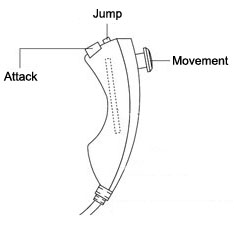
\includegraphics[scale=0.6]{Figures/nunchuk}
  \caption{Button specifications} 
  \label{fig:Nunchuk} 
\end{figure}
